%===========================================================
\chapter{Analytics and Evolutionary Observers}
%===========================================================

Observers measure the world without changing it: none consumes engine RNG and
none runs inside decision logic. They are what turn a moving picture into
evidence.

\section{Sampled metrics}
\code{MetricsRecorder} samples the population every \code{sample\_interval}
ticks: counts of animals and food patches, cumulative births and deaths, mean
energy and injury, environmental signals, food and metabolic multipliers, trait
means, a normalised diversity summary over a sample of \code{diversity\_sample}
animals, and development measures (deepest and mean living generation, founder
fraction, juvenile fraction, mean age). Missing measurements in older saves remain
\code{null} and are drawn as gaps, never as zero.

\section{Generation depth}
Generation is \emph{ancestral depth}, not a temporal cohort. An animal with no
recorded parents is generation 0; otherwise
\[
\text{gen}(x)=1+\max\big(\text{gen}(p_1),\text{gen}(p_2)\big).
\]
\code{LineageStore.generation\_of} traverses ancestry iteratively with cycle
detection and caches results; defining a new child invalidates only that child and
its descendants. Ancestry survives the deaths of ancestors and checkpoint restore.
The deepest living generation can fall when the deepest descendant dies.

\section{Exact birth-event Price decomposition}
At every birth event the recorder observes the entire pre-birth living population
of $n$ animals. For a trait $z_i$, let $w_i$ be the attributable offspring
contribution (0.5 per child for each parent, 0 for non-parents) and $z'_i$ the
weighted mean of its descendants' trait. Then
\begin{align*}
\text{selection}&=\mathrm{Cov}(w,z)/\bar w, &
\text{transmission}&=\overline{w(z'-z)}/\bar w,\\
\text{total change}&=\textstyle\sum w z'/\sum w-\bar z, &
\text{residual}&=\text{total}-\text{selection}-\text{transmission}.
\end{align*}
Each offspring is counted once overall despite two parents. The identity is exact
to floating-point rounding. Worked example: $z=(1,3)$, $w=(1,3)$, $z'=(2,4)$ gives
$\bar w=2$, $\bar z=2$, $\mathrm{Cov}(w,z)=1$, selection $0.5$, transmission
$(1\cdot1+3\cdot1)/2/2=1.0$ and total $(2+12)/4-2=1.5$. If total descendant weight
is zero, change is undefined rather than zero. The terms are birth-event
accounting, not a causal estimate: mutation, crossover and mate choice all
contribute, and survival between births is not included. The GUI keeps 180 recent
cohorts; checkpoints and \code{evolution.json} keep 512.

\begin{figure}[htbp]
\centering
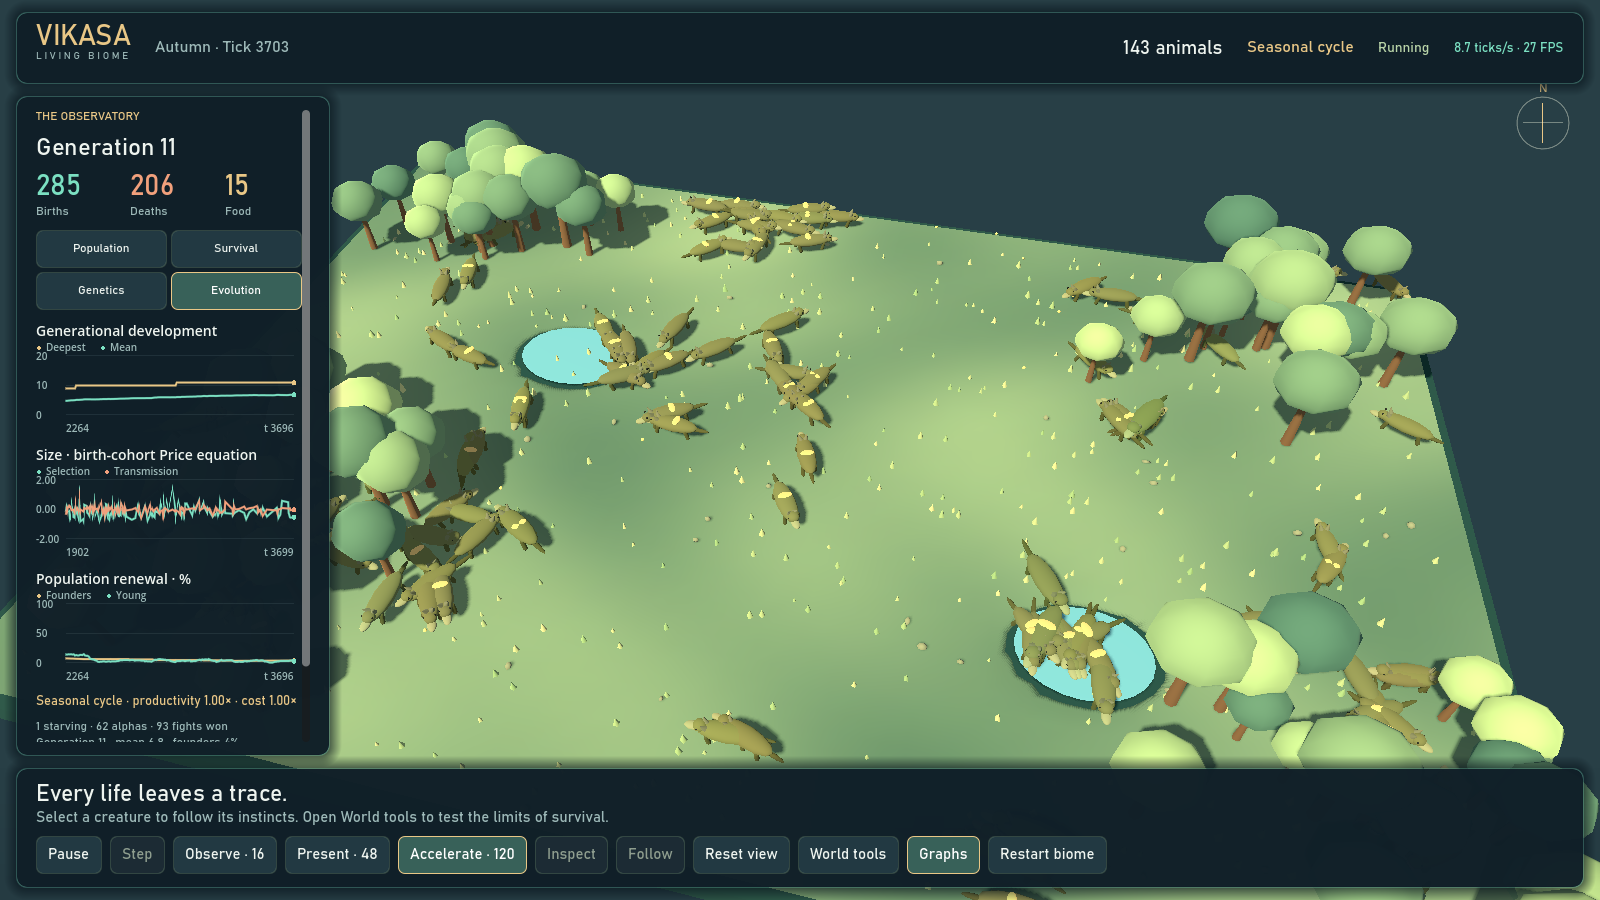
\includegraphics[width=0.92\textwidth]{research-evolution.png}
\caption{Evolution tab: generational development, signed birth-cohort Price
decomposition for size, and population renewal (founder and young fractions).}
\end{figure}

\section{Trait geometry}
At export, \code{analytics/trait\_space.py} normalises the living population's
traits to their fixed configured spans and computes
\begin{align*}
x_{ij}&=(z_{ij}-a_j)/(b_j-a_j), &
C&=(X-\bar X)^\top(X-\bar X)/(n-1),\\
R_{ij}&=C_{ij}/\sqrt{C_{ii}C_{jj}}, &
C\mathbf{v}_k&=\lambda_k\mathbf{v}_k,\quad f_k=\lambda_k/\textstyle\sum\lambda,\\
D_{\text{eff}}&=1/\textstyle\sum_k f_k^2 &&\text{(participation ratio, 1 to 6).}
\end{align*}
Eigenvectors come from NumPy \code{eigh}, sorted by descending variance, with signs
chosen so the largest-magnitude loading is positive; repeated eigenvalues are
flagged because tied axes have no unique orientation. Covariance and PCA are
unavailable below two individuals, constant columns have undefined correlations,
and non-finite or out-of-bounds clouds are rejected. $C$ is a phenotypic sample
covariance, not an additive genetic $G$ matrix, and each snapshot fits its own PCA
basis, so coordinates from different snapshots must not be connected.

\begin{figure}[htbp]
\centering
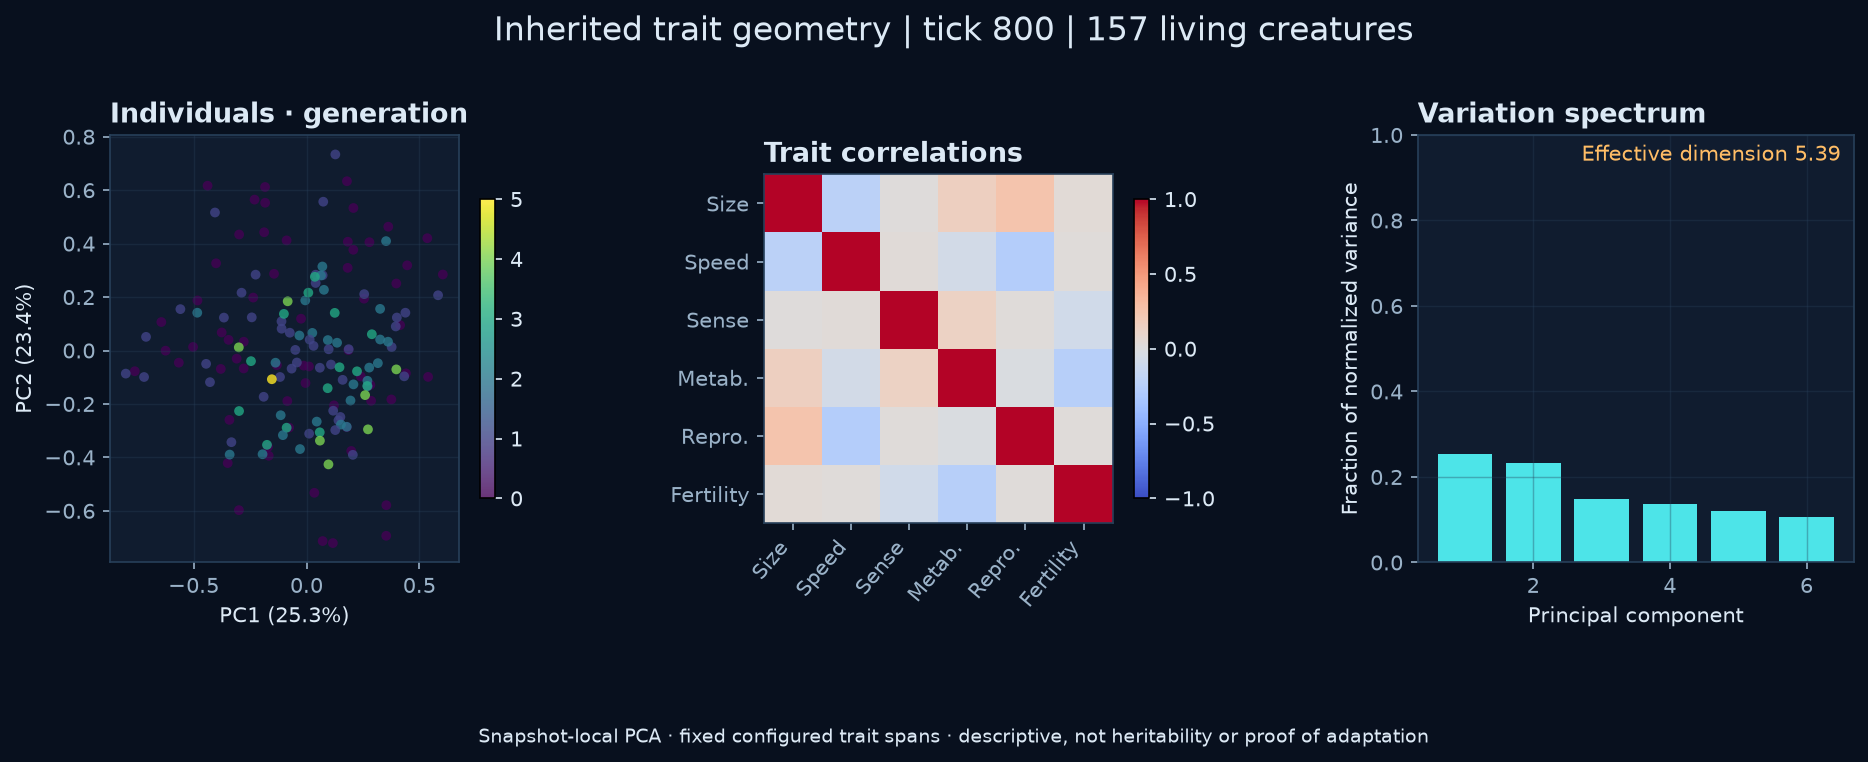
\includegraphics[width=0.95\textwidth]{trait-geometry.png}
\caption{Trait geometry, showcase seed 2026 at tick 800 (157 animals, deepest
generation 5): individuals on PC1/PC2 coloured by generation, trait correlations,
and the variance spectrum.}
\end{figure}

\section{Exported figures and how to read them}
\code{vikasa run} and \code{batch} write five static figures per run.

\begin{figure}[htbp]
\centering
\begin{minipage}{0.49\textwidth}\centering
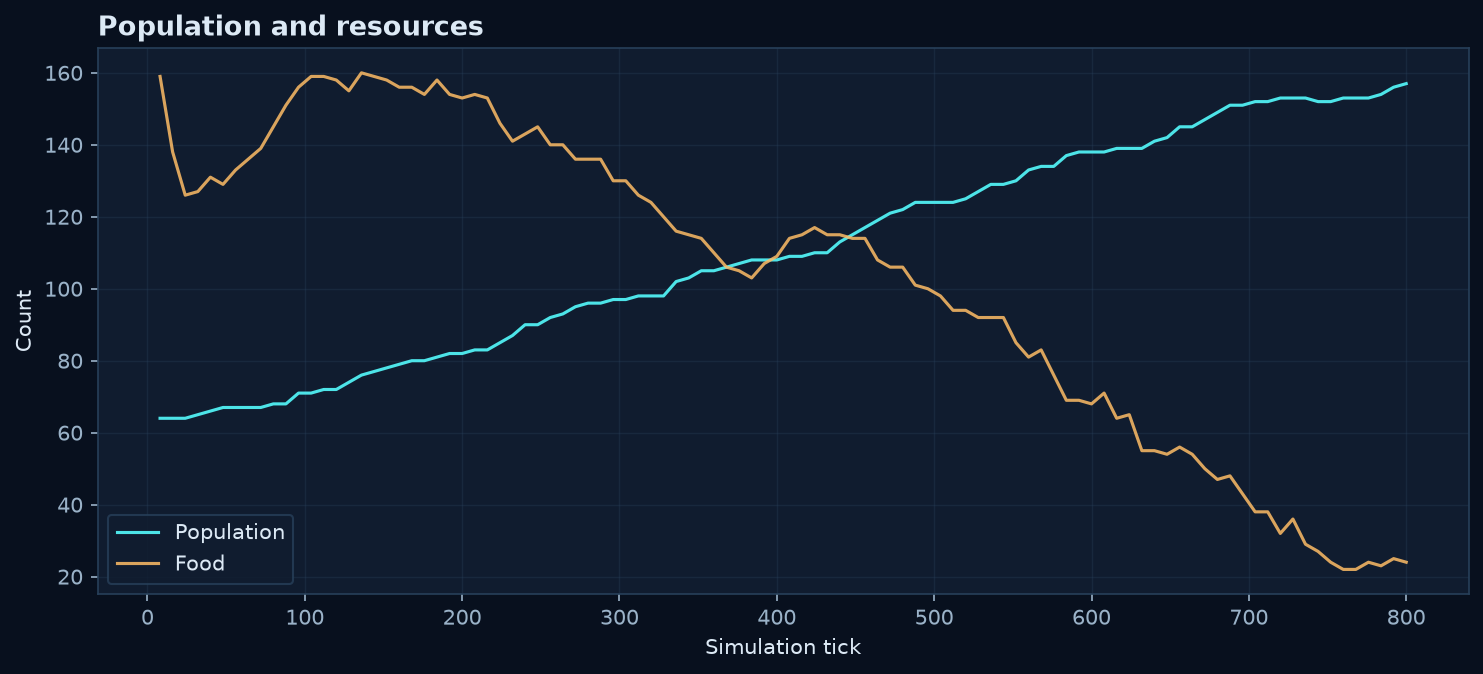
\includegraphics[width=\linewidth]{population.png}\\[-2pt]
{\small (a) Population and food patches}
\end{minipage}\hfill
\begin{minipage}{0.49\textwidth}\centering
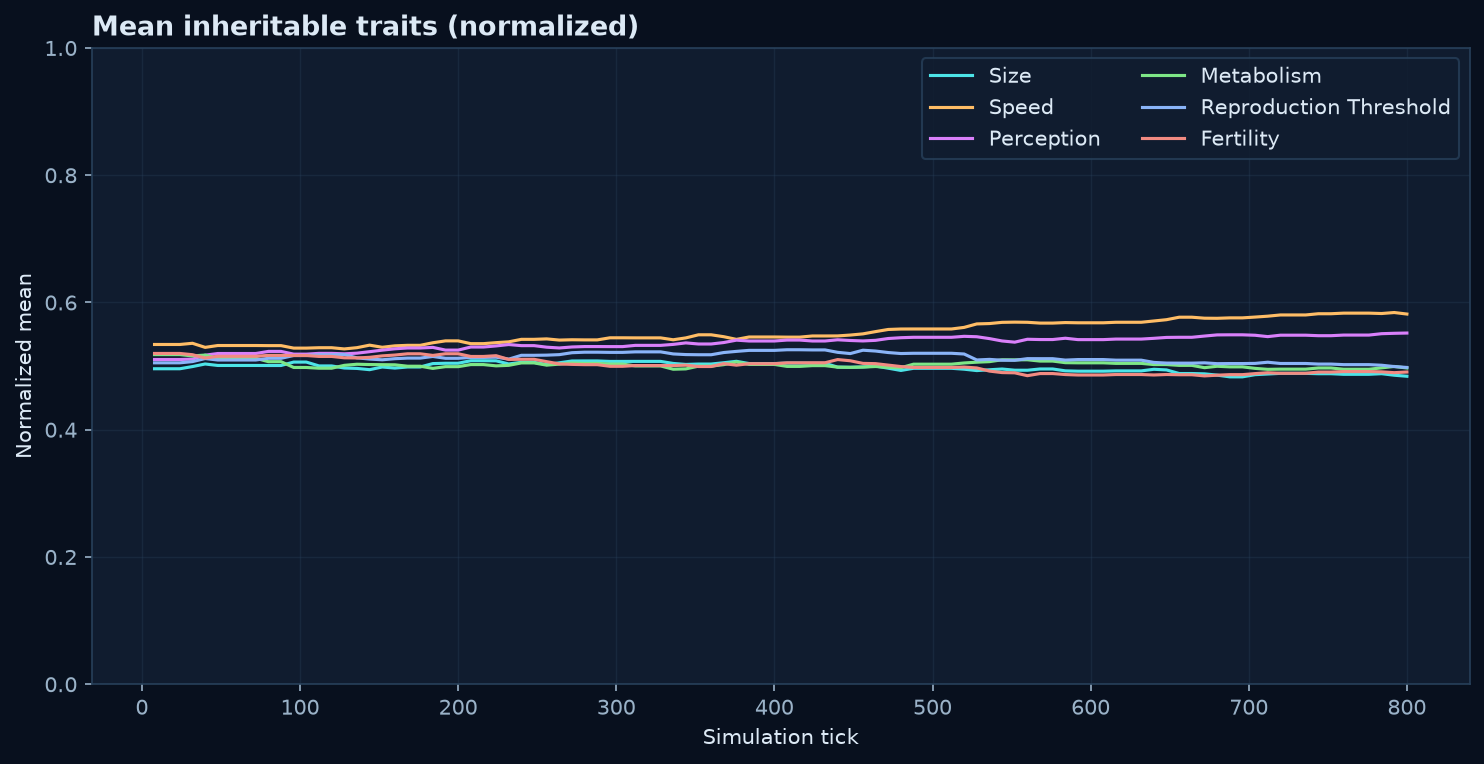
\includegraphics[width=\linewidth]{traits.png}\\[-2pt]
{\small (b) Normalised mean traits}
\end{minipage}\\[6pt]
\begin{minipage}{0.49\textwidth}\centering
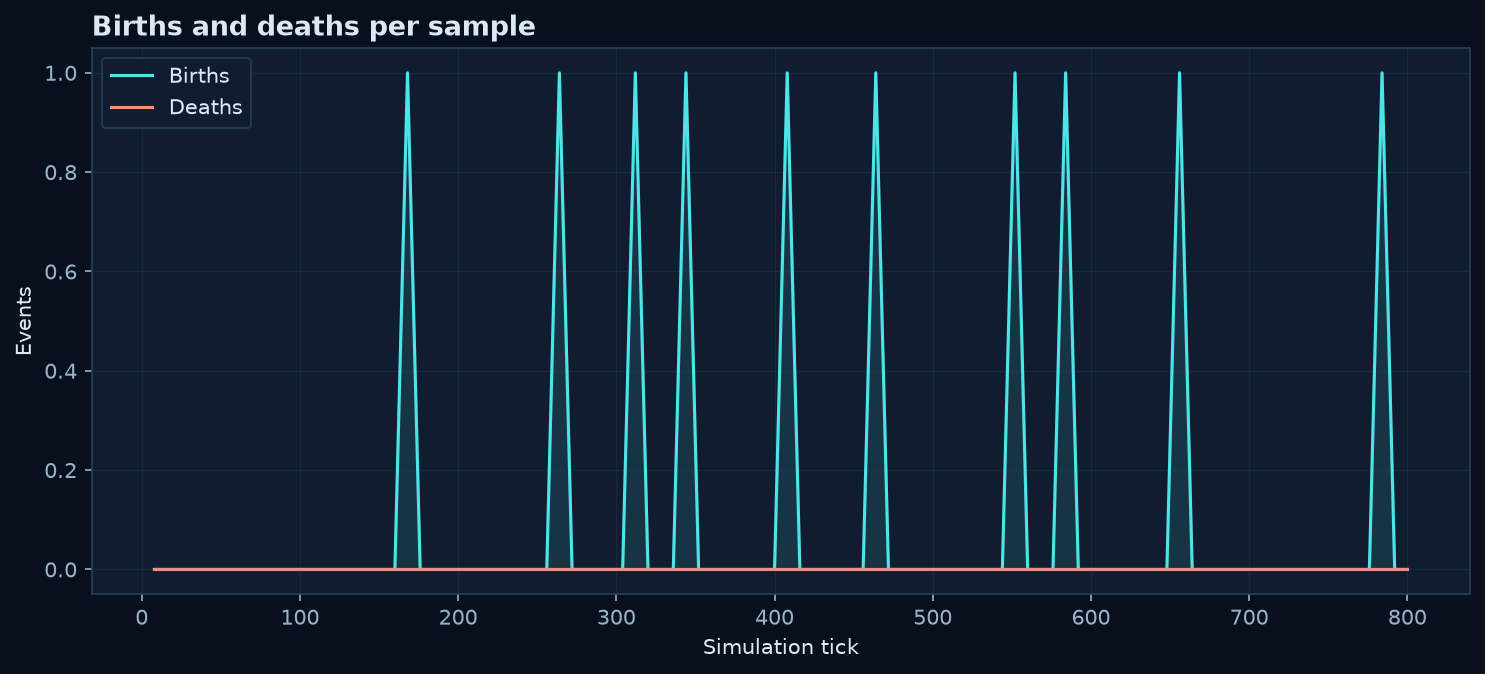
\includegraphics[width=\linewidth]{births_deaths.png}\\[-2pt]
{\small (c) Births and deaths at sample ticks}
\end{minipage}\hfill
\begin{minipage}{0.49\textwidth}\centering
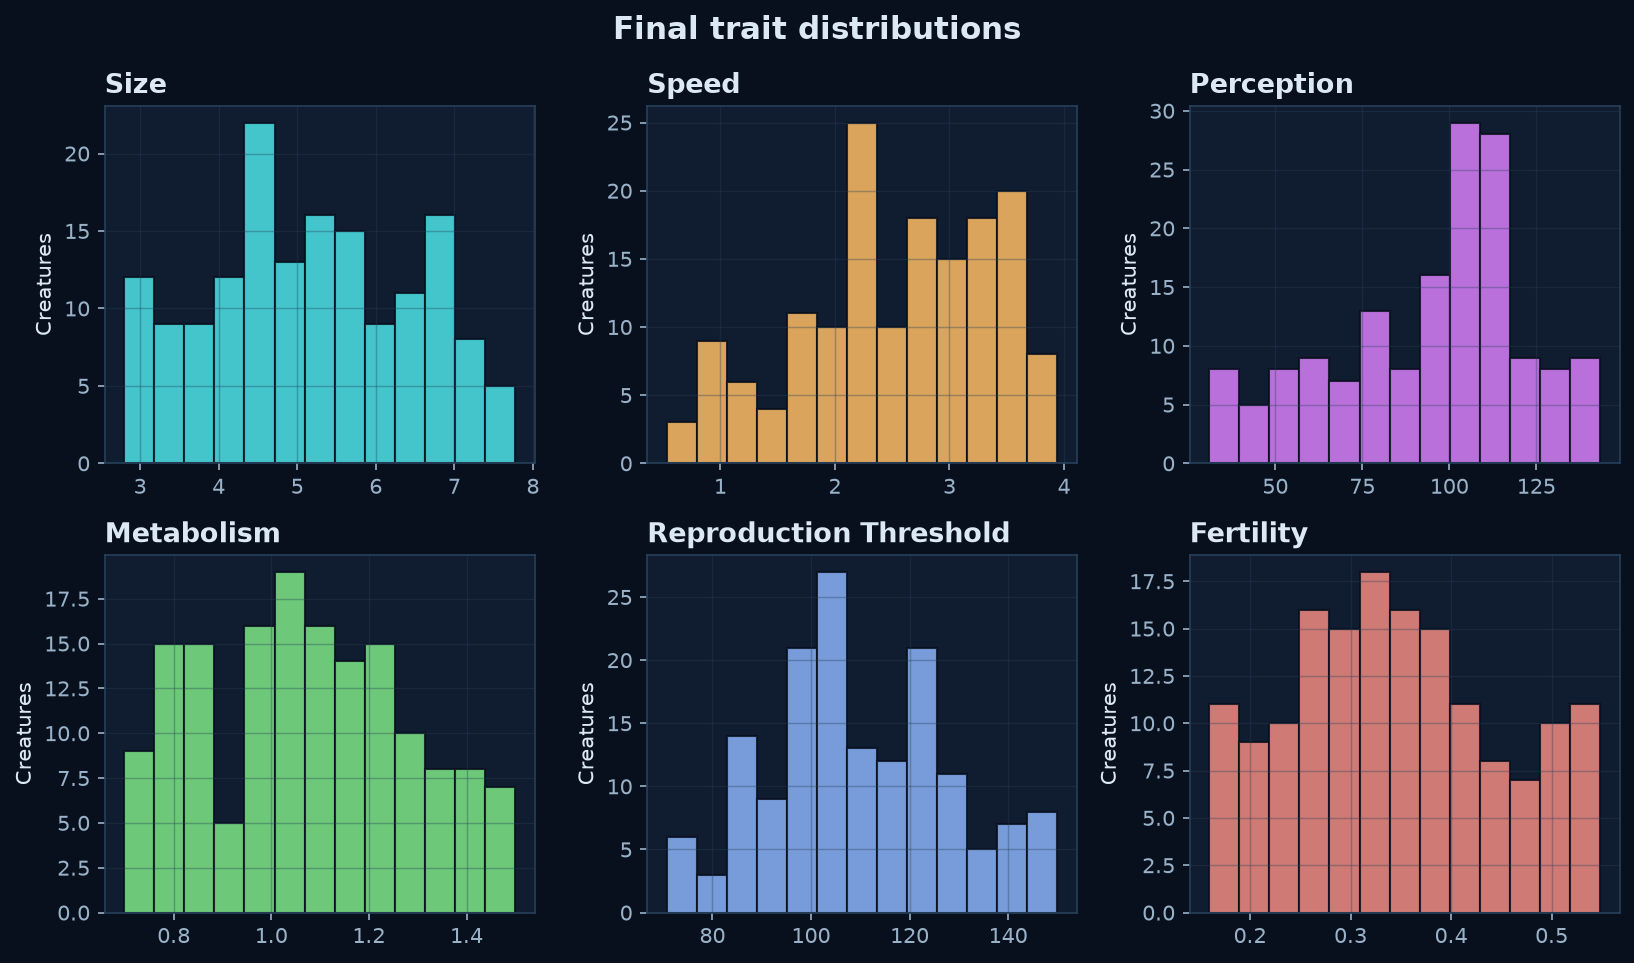
\includegraphics[width=\linewidth]{distributions.png}\\[-2pt]
{\small (d) Final trait distributions}
\end{minipage}
\caption{Exported figures for one showcase snapshot (seed 2026, tick 800).}
\end{figure}

\begin{itemize}[leftmargin=*]
\item \textbf{Ticks} are engine steps, not seconds. Requested speed is a target;
actual speed depends on hardware and population.
\item \textbf{Food-patch count} is not food energy or plant biomass.
\item \textbf{Normalised traits} $0.8$ mean 80\% through the configured range, not
80\% fitness; physical units differ between traits.
\item \textbf{Living-population means} change with births and deaths as well as
inheritance; a rising line alone does not prove adaptation.
\item \textbf{Births/deaths} in exported traces are events at the recorded sample
tick, not cumulative totals; use \code{total\_births} and \code{total\_deaths} in
the summary. For a closed run, $\text{living}=\text{founders}+\text{births}-\text{deaths}$.
\item \textbf{Weather shading} marks exposure, not proof of causation.
\item \textbf{Ribbons} in the experiment viewer are between-seed quartiles, not
confidence intervals.
\end{itemize}

\begin{table}[htbp]
\centering
\caption{Live Observatory graph groups}
\begin{tabularx}{\textwidth}{lL}
\toprule
Graph & Axes and interpretation \\
\midrule
Population \& food & Tick vs counts of animals and food patches. \\
Life \& loss (cumulative) & All births and deaths since the run began; never decrease within a run. \\
Energy \& injury & Population-mean reserve fraction and injury, as percentages. \\
Temperature \& rainfall & Normalised environmental indices (not $^{\circ}$C or mm, unless climate forcing is on). \\
Food \& metabolic pressure & Multipliers: food below $1\times$ reduces production; cost above $1\times$ raises expenditure. \\
Inherited size \& speed & Raw trait means; compare each line with itself. \\
Genetic diversity & Normalised summary of trait variation; not heterozygosity or heritability. \\
Evolution & Generation depth, renewal, signed Price terms per cohort. \\
Ecology & Plant/water fractions, reserves, cumulative flows and the cell map (spatial profile). \\
\bottomrule
\end{tabularx}
\end{table}

\section{Survival uncertainty: the Wilson interval}
For $k$ non-extinct runs out of $n$ seeds at a declared horizon, Vikasa reports
$p=k/n$ with a Wilson score interval ($z=1.959963984540054$):
\[
c=\frac{p+z^2/2n}{1+z^2/n},\qquad
h=\frac{z\sqrt{p(1-p)/n+z^2/4n^2}}{1+z^2/n},\qquad
[\max(0,c-h),\ \min(1,c+h)].
\]
This avoids reporting zero uncertainty when all of a few runs survive or die. For
$k=n=3$ it gives $[0.4385,1.0000]$, which is why three-seed studies are described
as exploratory throughout.

%===========================================================
\chapter{Headless Experiments and the Controlled Laboratory}
\label{ch:experiments}
%===========================================================

\section{Commands}
\begin{table}[htbp]
\centering
\caption{Headless science commands}
\begin{tabularx}{\textwidth}{lL}
\toprule
Command & Purpose \\
\midrule
\code{validate --config F} & Parse and validate a configuration. \\
\code{run --scenario S --output D [--seed --ticks]} & One scenario; CSV/JSON/PNG exports with hashes. \\
\code{batch --scenario S --output D --replicates 3} & Deterministic replicates with consecutive seeds. \\
\code{study --config F --seeds 2026 7 41 --ticks 12000} & Generational development study with Wilson interval. \\
\code{contrast --protocol P --output D} & Predeclared seed-blocked multi-condition comparison. \\
\code{stress --config F --ticks 100000 --seed 2026} & Long invariant-audited run. \\
\bottomrule
\end{tabularx}
\end{table}

An export directory contains \code{config.json}, \code{summary.json},
\code{metrics.csv}, \code{events.json}, \code{creatures.csv} (with generation
depth), \code{lineage.csv}, \code{evolution.json} (last 512 cohorts),
\code{trait-space.json}, \code{habitat.json} (spatial profile) and the figures
\code{population.png}, \code{traits.png}, \code{births\_deaths.png},
\code{distributions.png} and \code{trait\_space.png} (plus \code{chromosomes.png}
for diploid runs); every file's SHA-256 is recorded in the export manifest. A batch
writes one directory per replicate, \code{replicate-001-seed-<seed>}, using
consecutive seeds starting from the scenario seed.

\section{Development studies}
The \code{study} command records every selected seed, exact extinction times,
sampled trajectories, invariant errors, source and configuration hashes and a
Wilson survival interval. It never discards extinct runs, and it rejects
publication if source files change during execution.

\begin{table}[htbp]
\centering
\caption{Showcase development study, 12{,}000 ticks}
\begin{tabular}{lccccc}
\toprule
Seed & Living & Births & Living depth & \multicolumn{2}{c}{Deaths: starvation / senescence / fights} \\
\midrule
2026 & 123 & 799 & 23 & \multicolumn{2}{c}{560 / 142 / 38} \\
7 & 117 & 720 & 23 & \multicolumn{2}{c}{478 / 154 / 35} \\
41 & 114 & 717 & 20 & \multicolumn{2}{c}{477 / 158 / 32} \\
\bottomrule
\end{tabular}
\end{table}
All three passed invariant checks (Wilson $[0.4385,1.0000]$). The preserved
extinction control died out at ticks 2{,}870, 2{,}589 and 2{,}265 (Wilson
$[0.0000,0.5615]$). This is a multi-parameter comparison, not a causal estimate for
any single coefficient.

\section{Seed-blocked contrast protocol}
A contrast protocol declares a base configuration, the complete unique seed list,
horizon, sample interval, control identifier, bootstrap seed and resample count,
and every condition's overrides and events. Everything is validated before the
first tick: unknown fields, fractional or boolean seeds and times, duplicate IDs and
out-of-horizon events are rejected. Limits: 128 seeds, 8 conditions, $10^6$ ticks,
64 events per condition, 50{,}000 resamples and 250{,}000 stored records.

Extinction is absorbing, but plant and water processes continue to the same
horizon, so final water is never compared across different times. Failed runs keep
their condition, seed, stage, tick and exception, invalidate the affected
comparison, and make the CLI exit with status 1.

\subsection{Mathematics}
For condition $a$, control $c$, seed block $s$ and horizon $T$, with $N_{as}(t)$
the population after $t$ transitions:
\begin{align*}
I_{as}&=\textstyle\sum_{t=1}^{T}N_{as}(t)\ \text{[animal-ticks]}, &
M_{as}&=I_{as}/T,\\
D_s&=Y_{as}-Y_{cs}, &
\bar D&=\tfrac1n\textstyle\sum_s D_s,\\
s^2&=\tfrac{1}{n-1}\textstyle\sum_s(D_s-\bar D)^2, &
\mathrm{SE}&=\sqrt{s^2/n}.
\end{align*}
The seed block is the unit of replication. The paired bootstrap draws $n$ seed
indices with replacement, applies the same indices to both arms, and reports the
2.5th and 97.5th percentiles of the resampled means; a separate generator with the
declared bootstrap seed ensures it cannot alter biology. Hand-checked fixture: one
founder dying on transition 3 over 20 ticks has integral 2 and mean 0.1;
differences $[-2,0,2]$ give mean 0, variance 4 and SE $\sqrt{4/3}$.

\subsection{Evidence package}
Each run publishes \code{report.json}, an offline interactive \code{index.html}
(no network, no CDN, text inserted as text) and \code{manifest.json} with SHA-256
hashes. Output directories are claimed exclusively and \code{INCOMPLETE.txt} remains
until publication finishes. \code{.gitattributes} keeps LF endings so Windows
checkouts cannot invalidate byte hashes.

\begin{figure}[htbp]
\centering
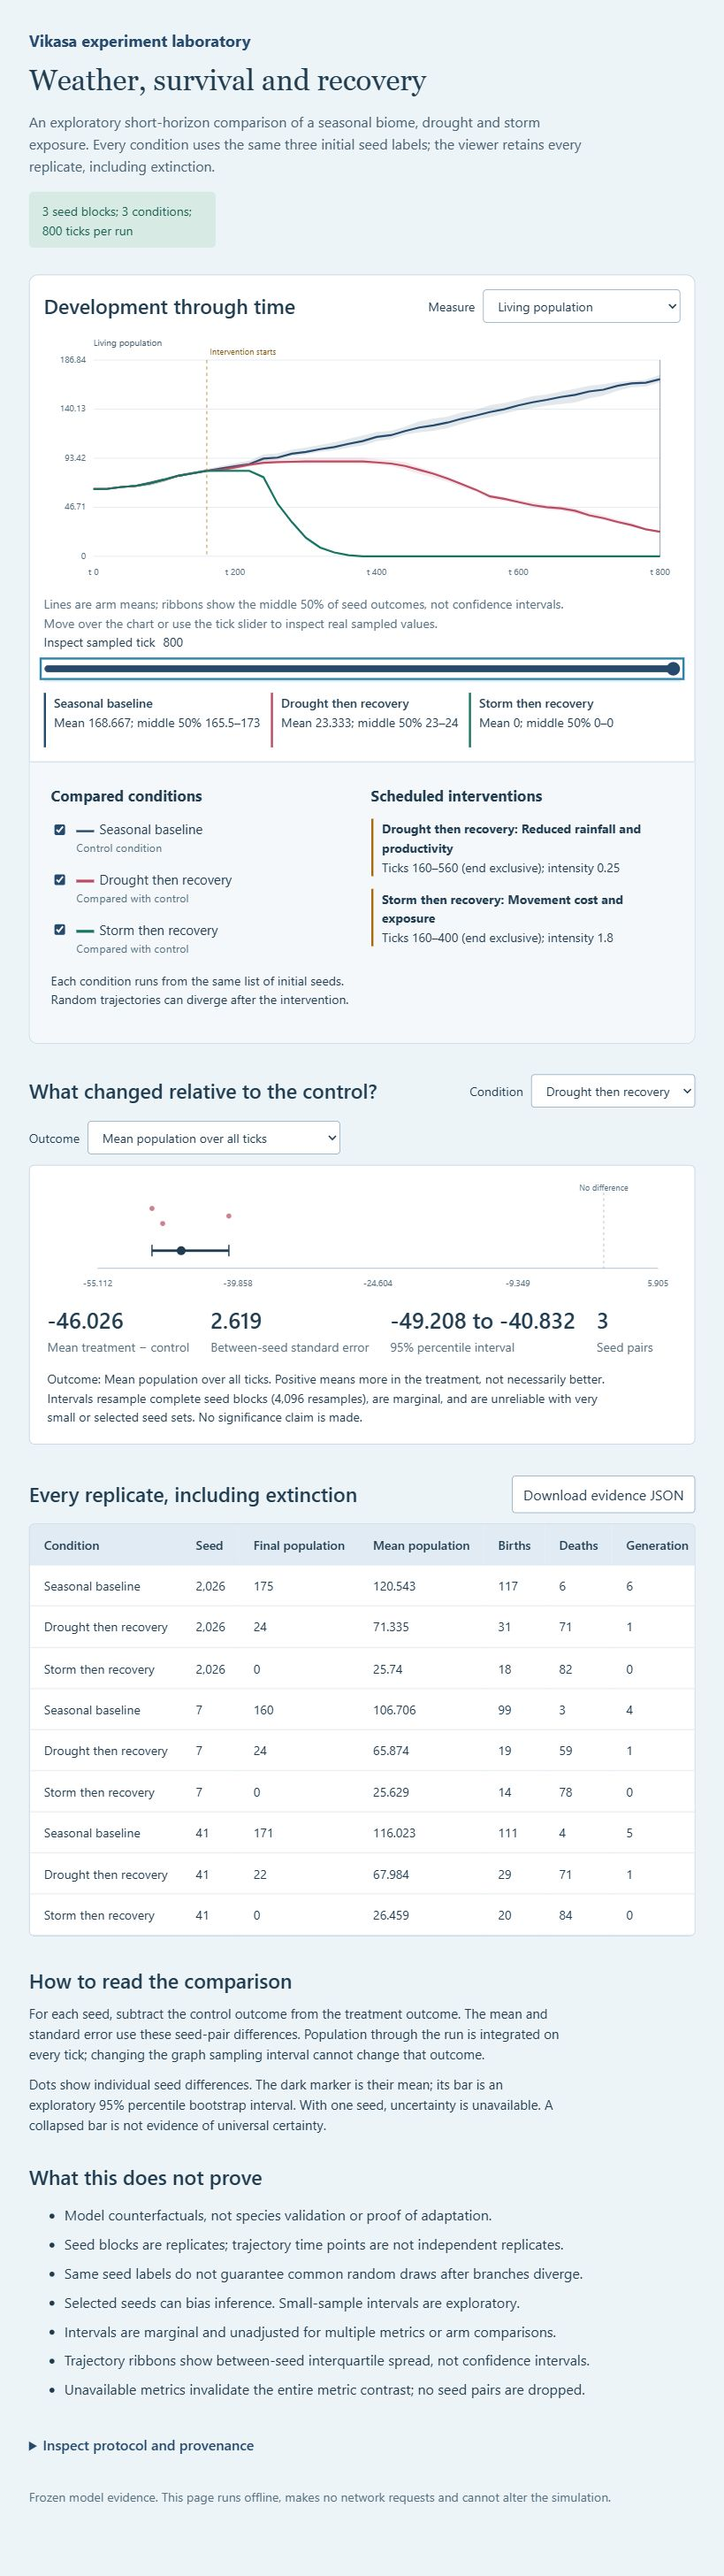
\includegraphics[width=0.9\textwidth]{controlled-experiments.jpg}
\caption{Offline weather-laboratory viewer: condition means with between-seed
quartile ribbons, intervention markers and paired effects.}
\end{figure}

\begin{table}[htbp]
\centering
\caption{Weather preview: 3 seeds $\times$ 3 conditions, 800 ticks}
\begin{tabular}{llcccc}
\toprule
Seed & Condition & Final population & Deaths & Deepest gen. & Extinction tick \\
\midrule
2026 & Baseline & 175 & 6 & 6 & --- \\
2026 & Drought & 24 & 71 & 1 & --- \\
2026 & Storm & 0 & 82 & 0 & 369 \\
7 & Baseline & 160 & 3 & 4 & --- \\
7 & Drought & 24 & 59 & 1 & --- \\
7 & Storm & 0 & 78 & 0 & 370 \\
41 & Baseline & 171 & 4 & 5 & --- \\
41 & Drought & 22 & 71 & 1 & --- \\
41 & Storm & 0 & 84 & 0 & 348 \\
\bottomrule
\end{tabular}
\end{table}
Relative to control, mean population over all ticks changed by $-46.026$ animals for
drought (paired percentile interval $[-49.208,-40.832]$) and $-88.481$ for storm
($[-94.803,-81.078]$). Storm intensity 1.8 is a severe model parameter bundle, not
a physical storm category, and drought changes rainfall, productivity, decay,
metabolism and exposure together, so the comparison estimates the configured
bundle, not an isolated mechanism. A larger eight-seed, 3{,}000-tick protocol
(\code{experiments/weather-contrast.json}) is provided for prospective execution.
